\providecommand{\main}{../../../..}
\documentclass[\main/dresen_thesis.tex]{subfiles}
\begin{document}
  \label{sec:doublelayers:layers:pnr}
  \begin{figure}[tb]
    \centering
    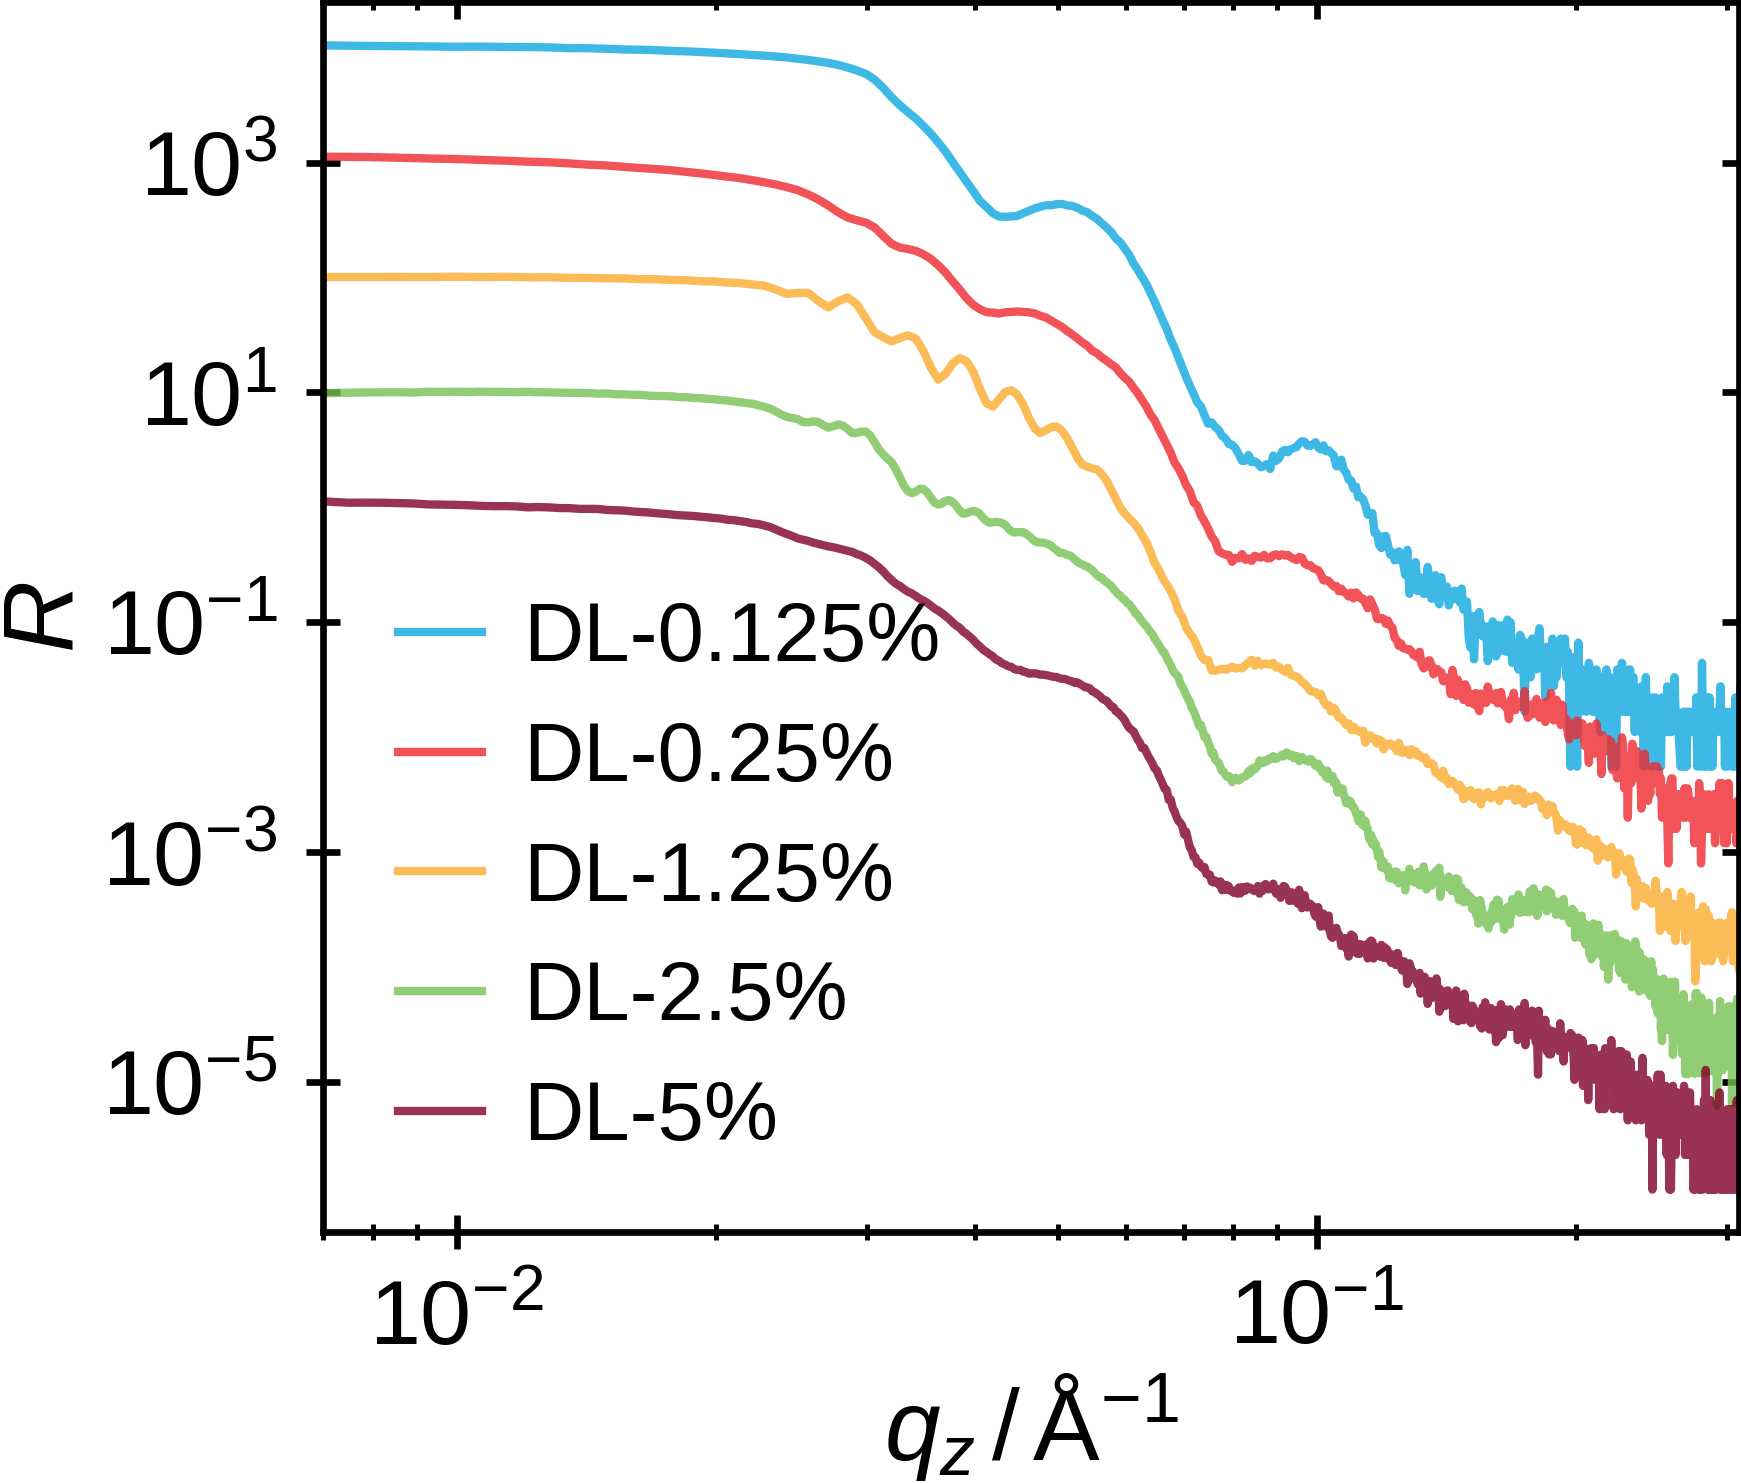
\includegraphics{doubleLayers_XRR_compareThickness}
    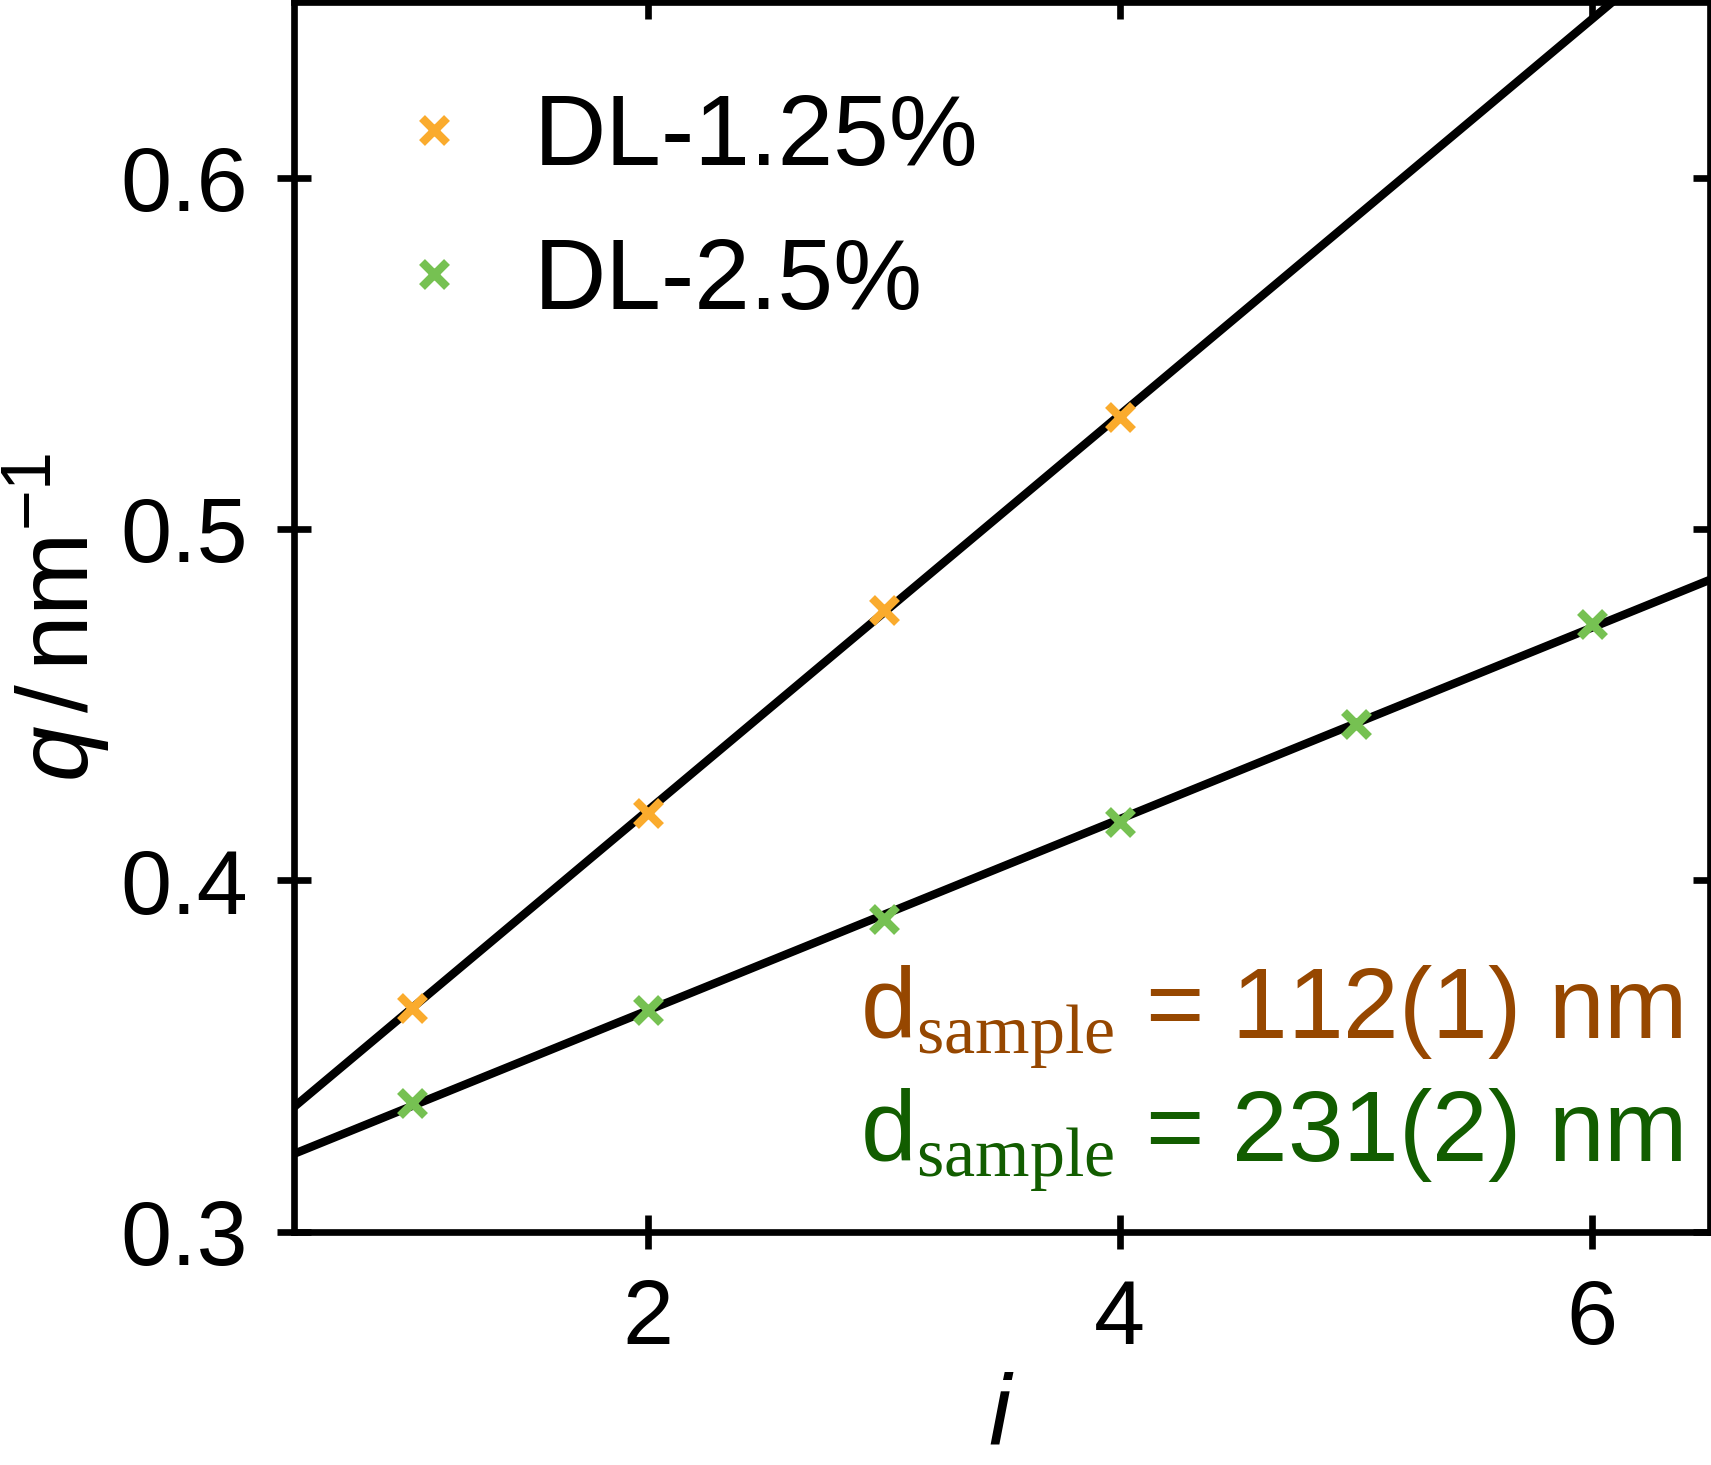
\includegraphics{doubleLayers_XRR_MinimaPositions}
    \caption{\label{fig:doublelayers:xrr:thicknessComparison}X-ray reflectivity (left) of double layer samples DL-0.125\%, DL-0.25\%, DL-1.25\%, DL-2.5\% and DL-5\%, which vary in the thickness of the PMMA spacer layer between the nanocube layers. Additionally marked by black vertical lines are the estimated peak positions visible in every sample from the nanocube thickness. For the samples DL-1.25\% and DL-2.5\% with well defined Kiessig fringes, linear fits through the minima positions of the fringes are performed to estimate the sample thickness (right).}
  \end{figure}
  By measuring the specular reflection of X-rays, the two length scales in the double layer samples are aimed to be quantified.
  \reffig{fig:doublelayers:xrr:thicknessComparison} shows the XRR of the samples with varied spacer thickness in direct comparison in a double logarithmic plot.
  For DL-1.25\% and DL-2.5\% thin film oscillations (Kiessig fringes) are visible in the $q$-range between $0.2 - 0.6 \unit{nm^{-1}}$.
  For DL-0.25\% they are vaguely perceptible and for DL-0.125\% and DL-5\% they are not well defined.
  The Kiessig fringes connect to the sample thickness and by evaluating the minima positions, it can be estimated by a linear fit, which results in $112(1) \unit{nm}$ for DL-1.25\% and $231(2) \unit{nm}$ for DL-2.5\%.

  The broader peaks with the longer period visible in all reflectivity data sets on the other hand correspond to the nanocube layer thickness of the double layers.
  Evaluating the period qualitatively, an estimated thickness of $16(1) \unit{nm}$ is determined, which is tendentiously in the order of the nanocube size, including the oleic acid ligand shell around it.
  It is slightly larger by $1 - 2 \unit{nm}$, which is connected to the roughness of the layers induced by interfacial roughness and the particle size distribution.

  \begin{figure}[tb]
    \centering
    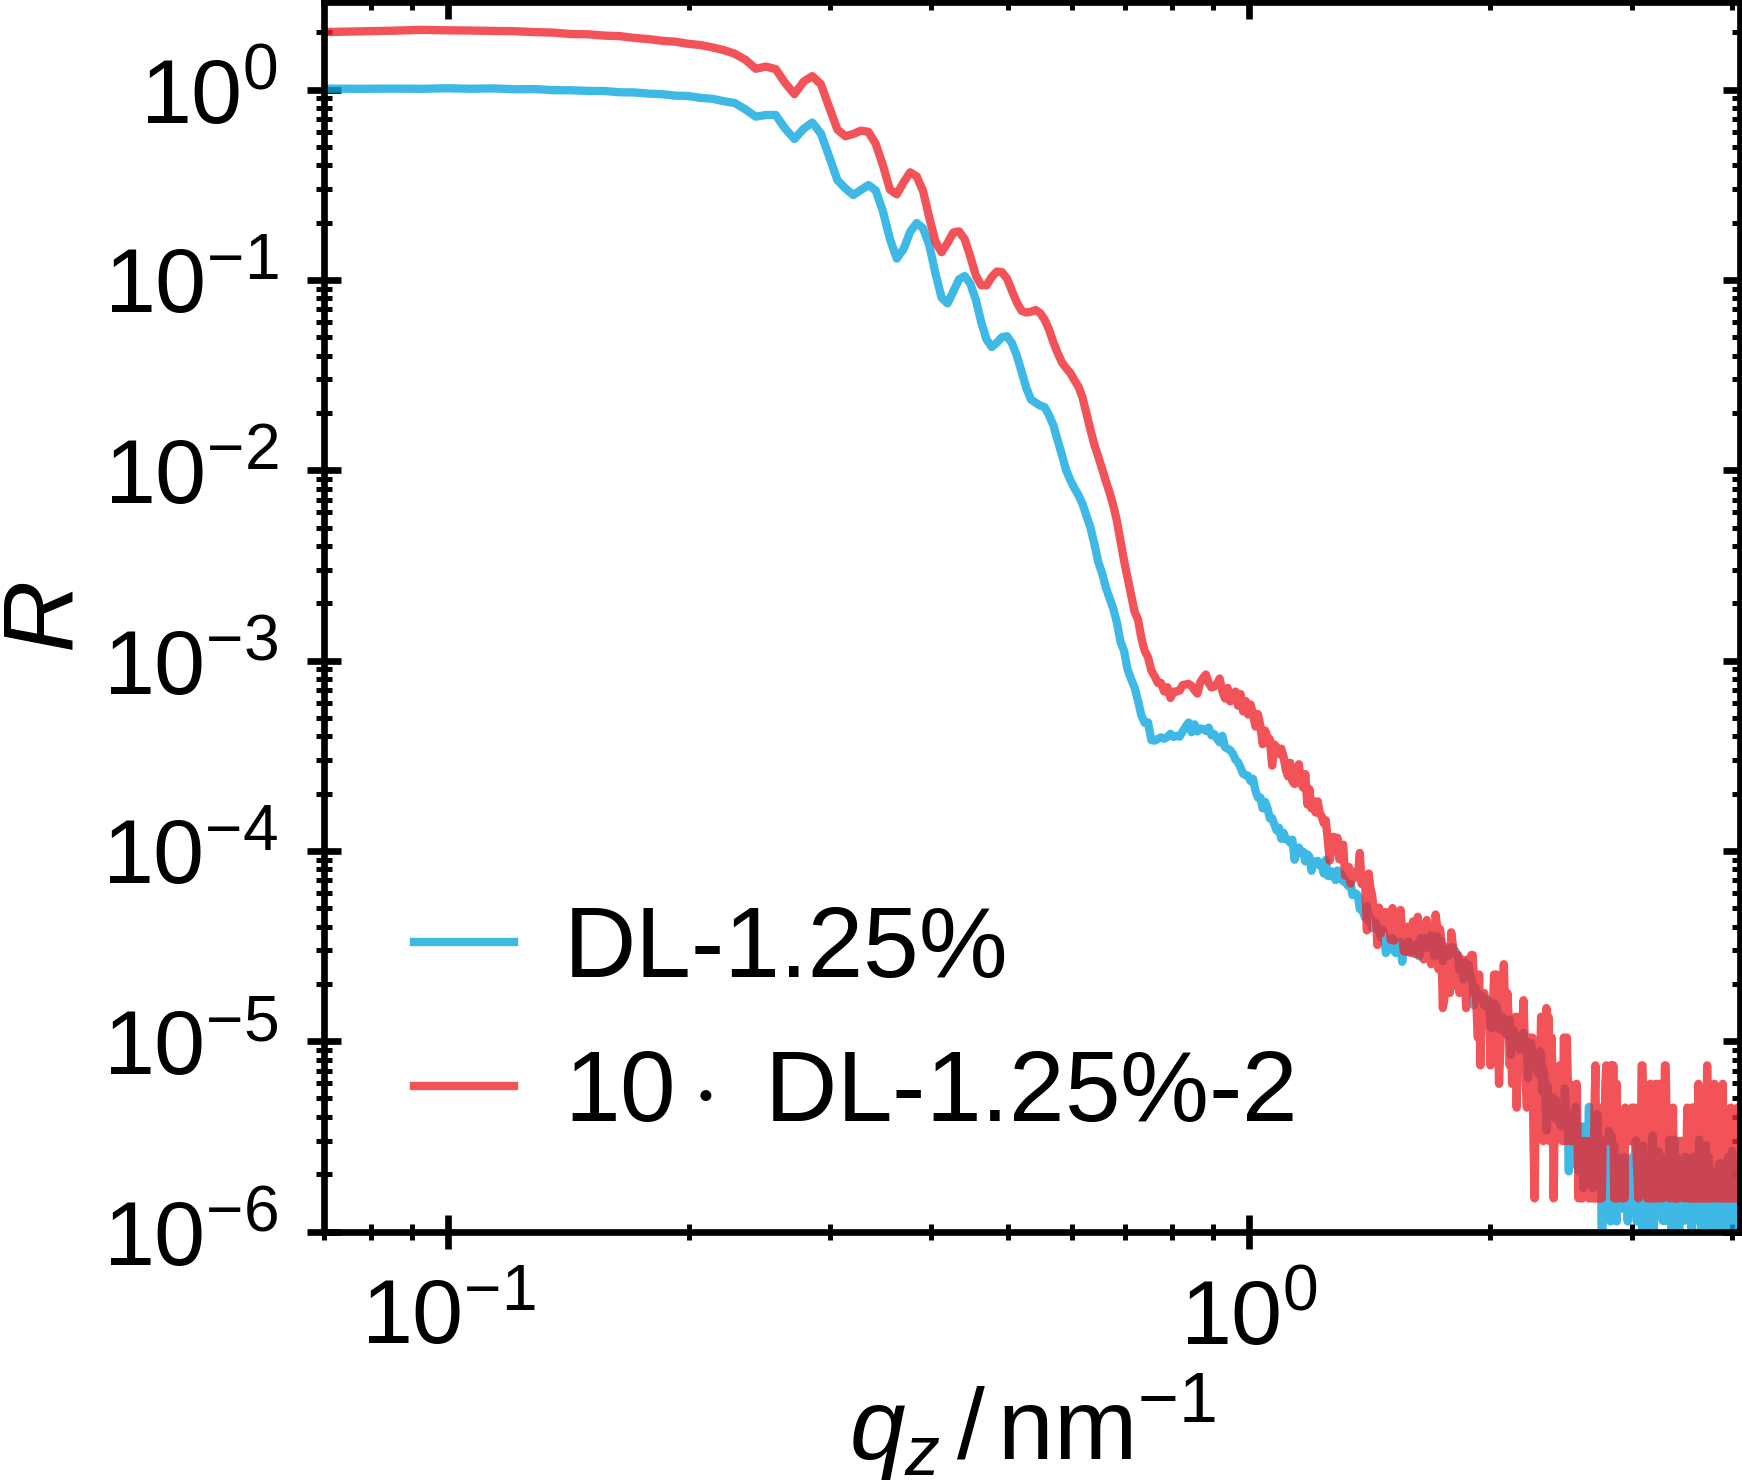
\includegraphics{doubleLayers_XRR_reproducibility}
    \caption{\label{fig:doublelayers:xrr:reproducibility}XRR of DL-1.25\% and DL-1.25\%-2, which were prepared in parallel using the same dispersions and environmental conditions. The reflectivity of DL-1.25\%-2 is shifted by a factor of two for visibility.}
  \end{figure}

  X-ray reflectometry is further use to show that the thickness of the sample is well reproducible when the same sample is produced multiple times.
  In \reffig{fig:doublelayers:xrr:reproducibility} the reflectivity of DL-1.25\% and DL-1.25\%-2 is shown, which were both prepared by the same conditions.
  Qualitatively the two data sets are very similar, with Kiessig fringes of the same periodicity, which shows that the same sample thickness is achieved in both cases.
  However, DL-1.25\%-2 drops off faster in reflectivity with respect to the scattering vector, which indicates a slightly higher roughness in the sample.
  Therefore a certain variability in the nanoparticle layer quality remains from the drop casting preparation, which is probably the reason as to why the XRR reflectivity data can not be simply described by the same nanoparticle profile, but has to be fit individually in each case.


  \begin{figure}[tb]
    \centering
    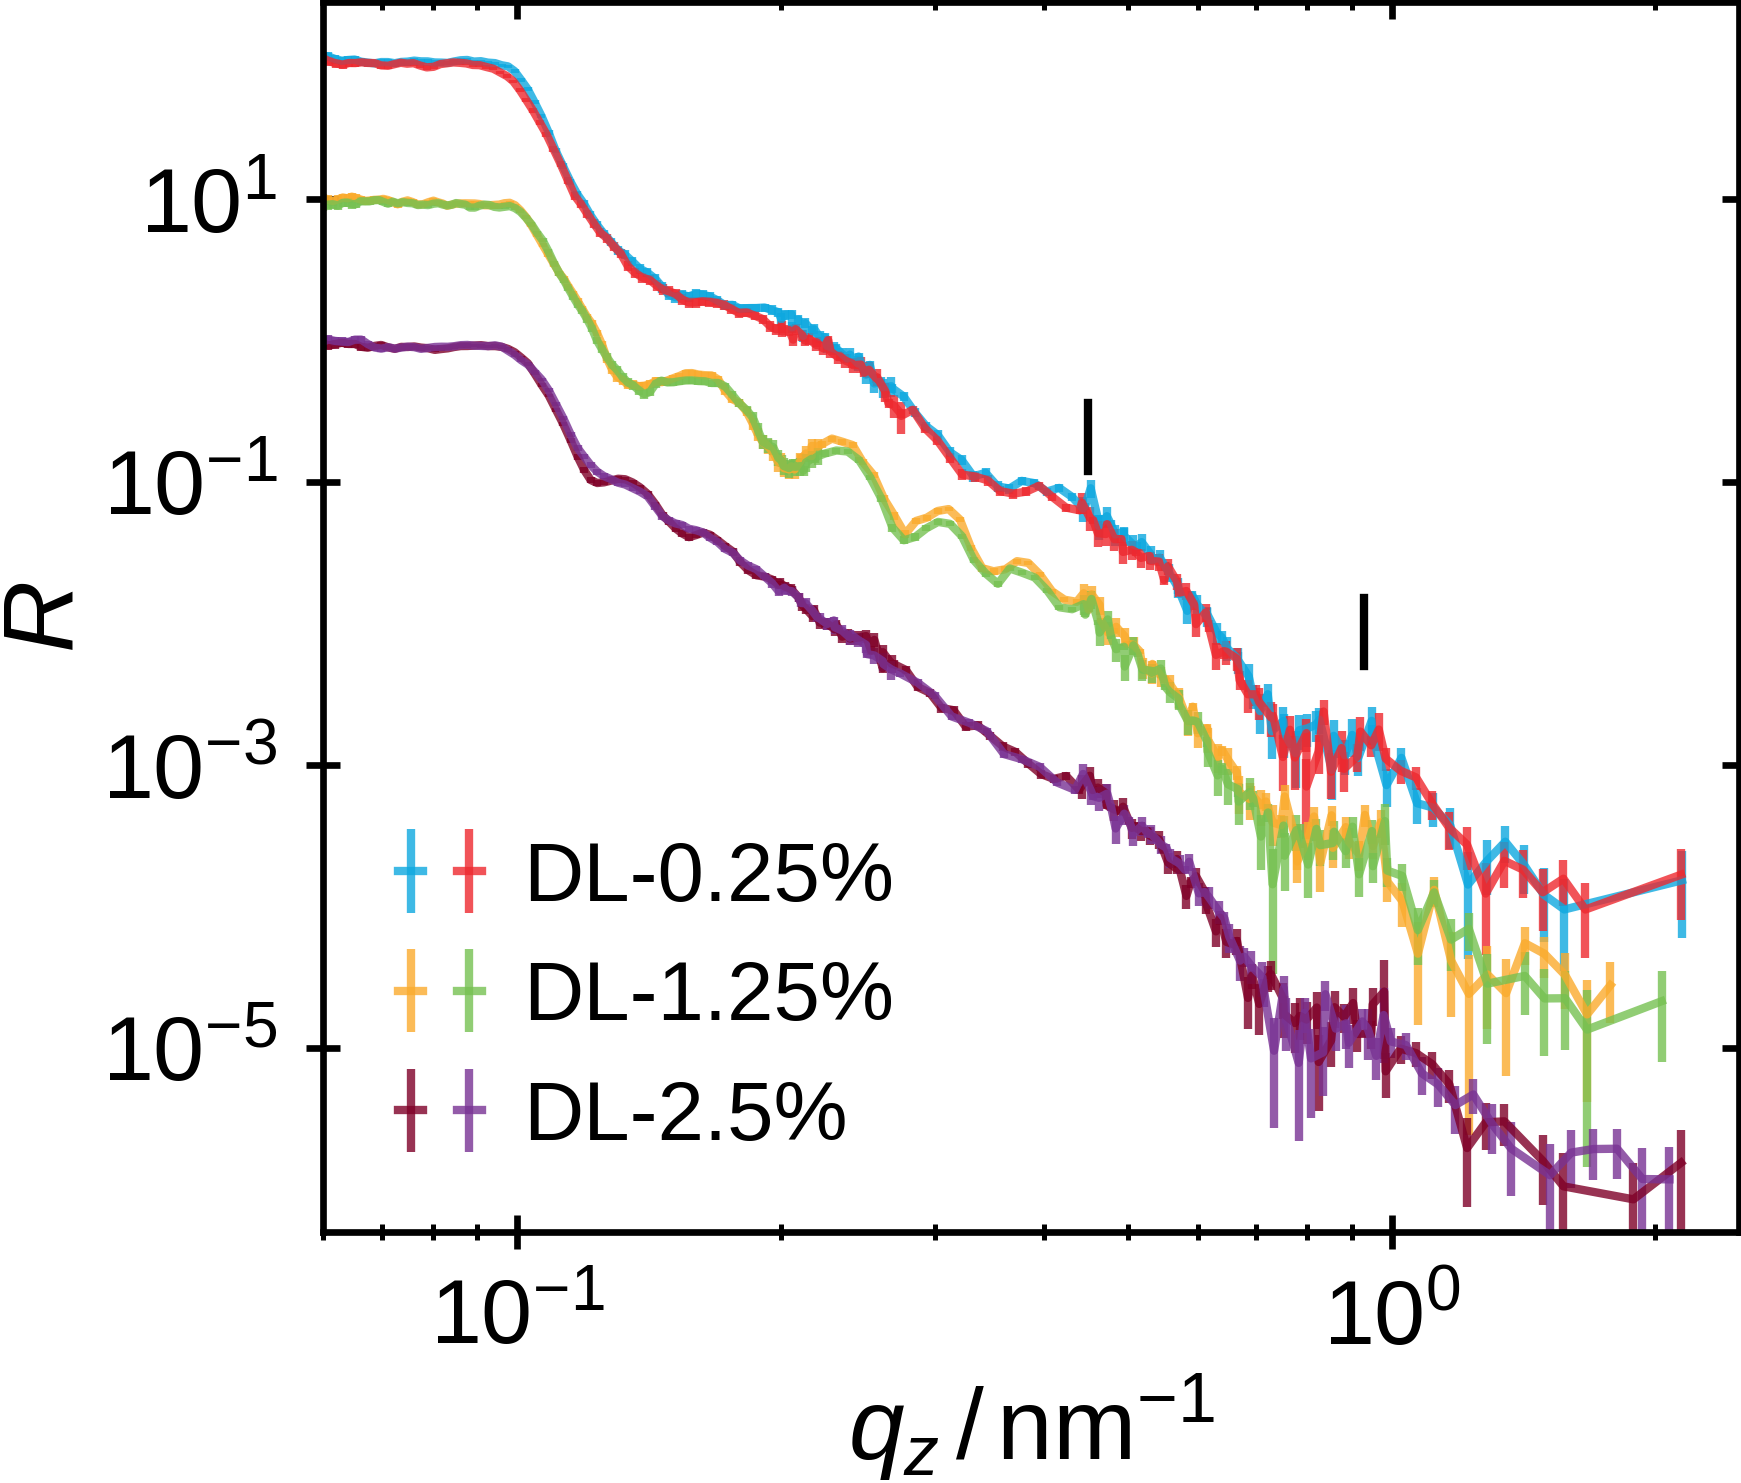
\includegraphics{doubleLayers_NR_compareThickness}
    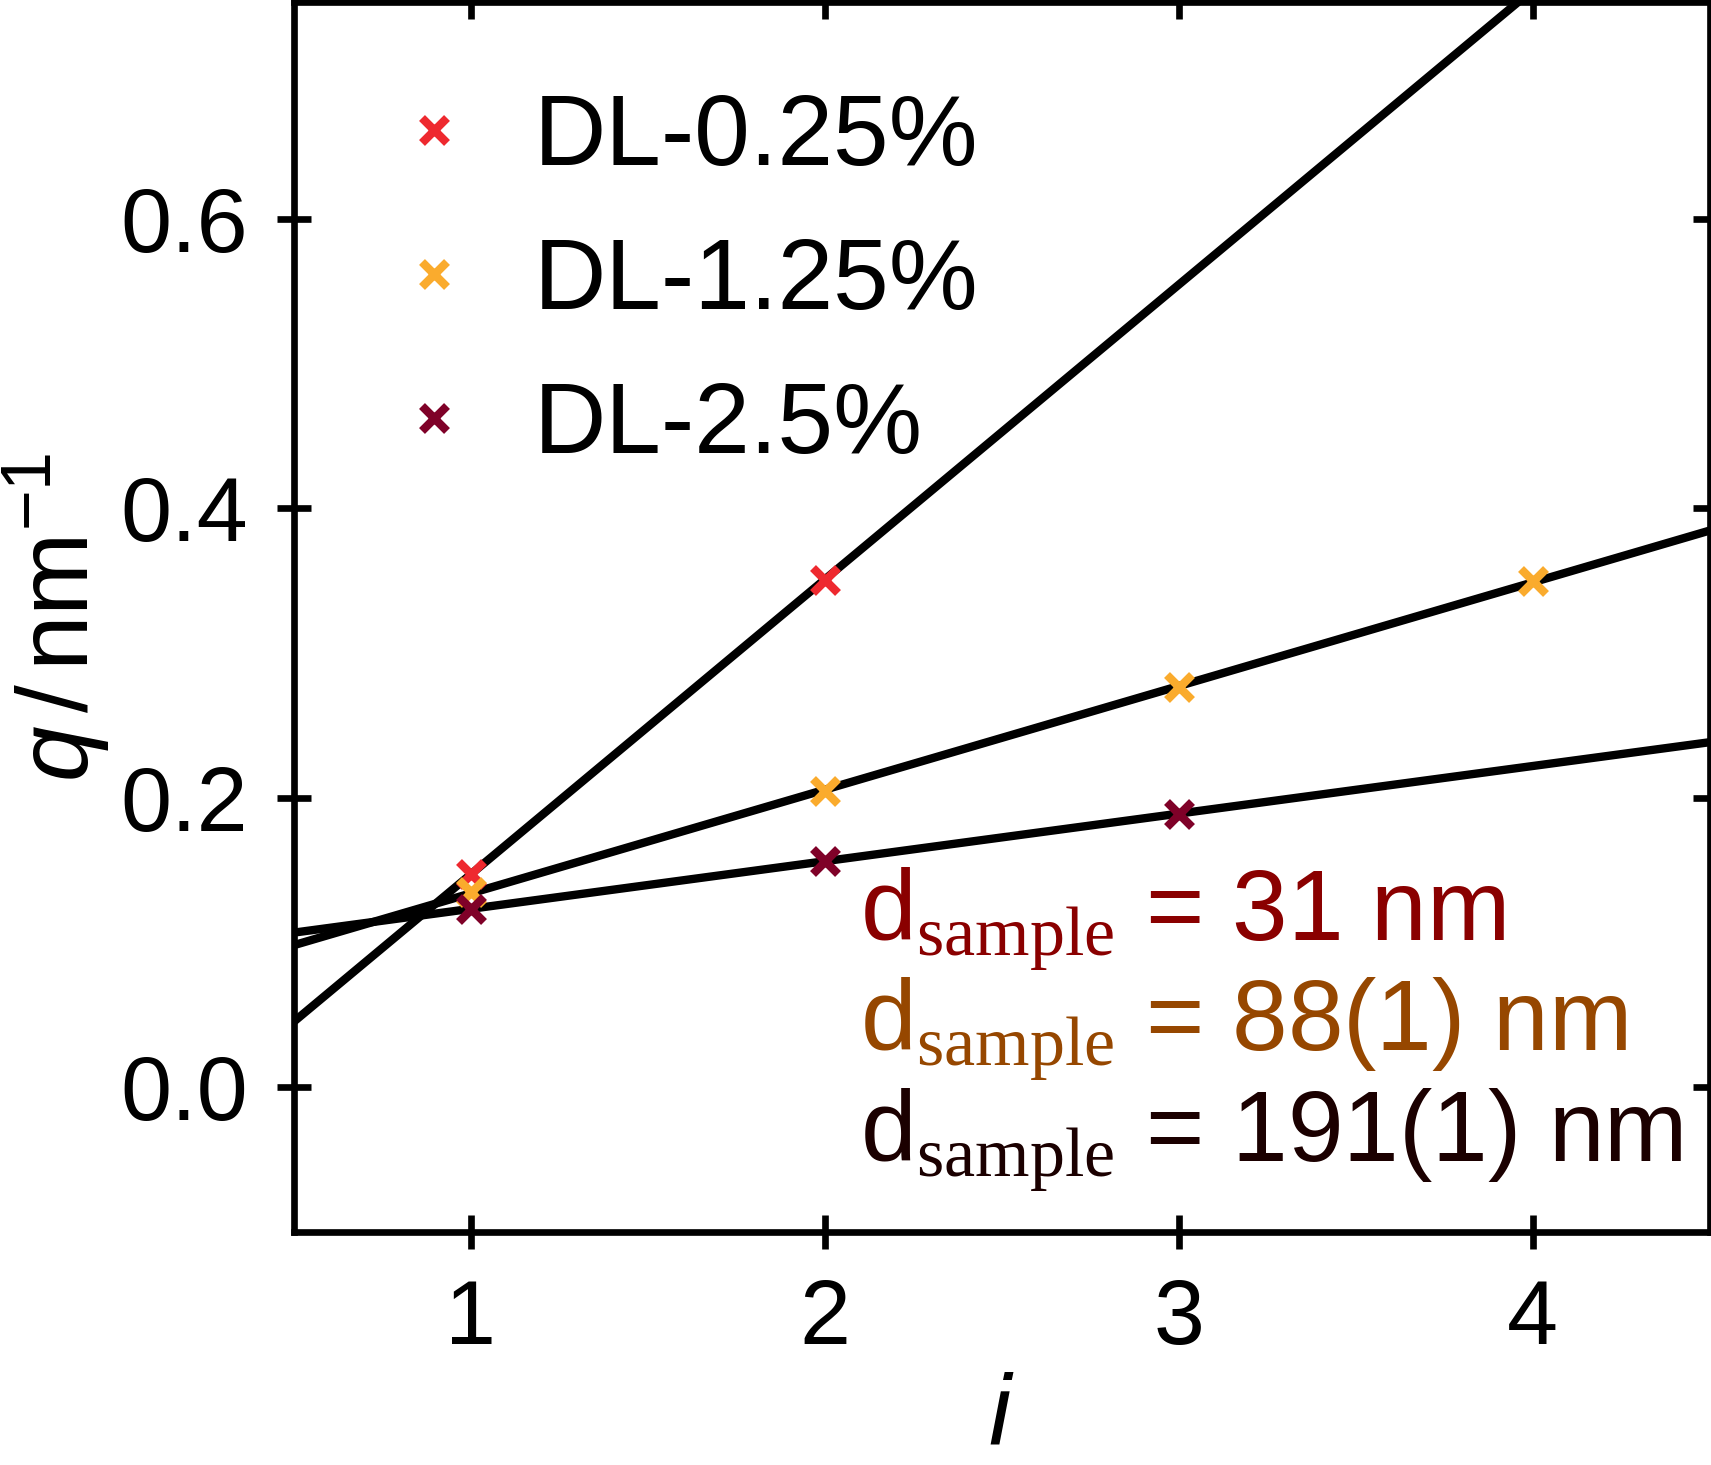
\includegraphics{doubleLayers_NR_MinimaPositions}
    \caption{\label{fig:doublelayers:nr:thickness}Neutron reflectivity (left) measured after zero-field cooling at guide field of DL-0.25\%, DL-1.25\% and DL-2.5\%. Analogue to \reffig{fig:doublelayers:xrr:thicknessComparison} the estimated peak positions visible from the nanocube thickness are marked by black vertical lines. The well-defined Kiessig fringe minimas are linearly fit to estimate the total sample thickness (right).}
  \end{figure}

  For DL-0.25\%, DL-1.25\% and DL-2.5\% polarized neutron reflectivity was obtained after zero-field cooling at the D17 instrument at ILL at $5 \unit{K}$ and is shown in \reffig{fig:doublelayers:nr:thickness}.
  Again Kiessig fringes are visible in all three cases, from which the sample thickness is determined from performing a linear fit through the observed minima to obtain the periodicity.
  A thickness of $31 \unit{nm}$, $88(1) \unit{nm}$ and $191(1) \unit{nm}$ is obtained respectively.
  For DL-0.25\% only two minima are observed, as to why no error estimation is given.
  Also visible in the neutron reflectivity is the length scale of the nanocube thickness in each sample.
  From the estimated peak positions of two peaks a thickness of $13(2) \unit{nm}$ can be estimated qualitatively.

  The observed thickness from SEM, XRR and NR are tabulated for comparison in \reftab{tab:doublelayers:ThicknessComparison}.
  In all three cases, the smallest thickness is observed by SEM, and the sample thickness from XRR is the largest.
  The value from SEM is the least reliable one, as the thickness from the SEM micrographs is obtained after violent breaking of the sample and it can not be excluded that the electron beam dissolved the PMMA layer partially during scanning of the sample.
  Due to the large discrepancy with XRR and NR, it should only be considered as to give an idea for the order of magnitude.
  The thickness obtained by the non-invasive macroscopic average from X-ray and neutron reflectivity is a more reliable source to quantify the sample thickness.
  However, also here a difference is observed in the Kiessig fringes period between the neutron reflectivity at $5 \unit{K}$ in comparison to XRR at room temperature.
  For DL-1.25\% the larger period in the Kiessig fringes of the neutron reflectivity translates to a reduced thickness of $24 \unit{nm}$ and for DL-2.5\% even to $40 \unit{nm}$.

  To estimate the interlayer distances in the samples, the estimated thickness of the nanocube layers as determined by SEM, XRR and NR is subtracted from the determined total sample thickness, respectively, in \reftab{tab:doublelayers:ThicknessComparison}.
  Similar to the sample thickness, smaller values are obtained for the interlayer spacing from the low-temperature NR in comparison to the XRR measurement, which correspond to a contraction of $23(2) \%$ and $17(1) \%$.
  The linear thermal expansion coefficient of PMMA is in the order of $10^{-4} \unit{K^{-1}}$ \cite{Michel_1986_Therm} and decreases with decreasing temperature to the order of $5 \cdot 10^{-7} \unit{K^{-1}}$ at $5 \unit{K}$ \cite{Lyon_1979_Tunne}.
  Thus for a temperature difference of $\Delta T \eq 290 \unit{K}$, thermal contraction accounts for less than $3 \%$ of the observed difference.
  For a better estimate of the layer distances that accounts for the varying contrast in the samples, instrumental resolution, \textit{etc.}, a quantitative evaluation of the data in the future by a scattering length density profile should give more precise data.

  \begin{table}[!htbp]
    \centering
    \caption{\label{tab:doublelayers:ThicknessComparison}Mean sample thickness as determined by SEM, XRR and NR in direct comparison. An estimate of the interlayer distance is given for SEM by subtracting the linear offset of $14(8) \unit{nm}$, and for XRR and NR by subtracting two times the estimated nanocube layer thickness of $16(1) \unit{nm}$ and $13(2) \unit{nm}$ respectively.}
    \begin{tabular}{ c | l | l | l }
      \rule{0pt}{2ex} \textbf{Thickness}  & $d_\mathrm{SEM} \, / \unit{nm}$ & $d_\mathrm{XRR} \, / \unit{nm}$& $d_\mathrm{NR} \, / \unit{nm}$ \\
      \hline
      DL-0.25\%  & $27(3)$  &           & $31$\\
      DL-1.25\%  & $72(3)$  & $112(1)$  & $88(1)$\\
      DL-2.5\%   & $154(4)$ & $231(2)$  & $191(1)$\\
      \hline
      \rule{0pt}{2ex} \textbf{Interlayer Distance}\\
      \hline
      DL-0.25\%  & $13(9)$  &           & $5(4)$\\
      DL-1.25\%  & $58(9)$  & $80(2)$   & $62(4)$\\
      DL-2.5\%   & $140(9)$ & $199(3)$  & $165(4)$\\
      \hline
    \end{tabular}
  \end{table}
\end{document}